\documentclass[t]{beamer}
\usetheme[deutsch]{KIT}
\setbeamercovered{transparent}
\setbeamertemplate{navigation symbols}{}

\KITfoot{Tutoriumsmaterial von Alexander Kwiatkowski, Michael Vollmer und Matthias Holoch \hspace{2.5cm} Basierend auf den Folien von Simon Stroh und Moritz v. Looz}
\usepackage[utf8]{inputenc}
\usepackage{amsmath}
\usepackage{ifthen}
\usepackage{amssymb}
\usepackage{tikz}
\usepackage{ngerman}
\usepackage[normalem]{ulem}
\usetikzlibrary{automata}
\usenavigationsymbols


\title{Theoretische Grundlagen der Informatik}
\subtitle{Tutorium}
\author{Alexander Kwiatkowski, Michael Vollmer und Matthias Holoch}

\institute[IKS]{Institut für Kryptographie und Sicherheit}

\TitleImage[height=\titleimageht]{images/tmaschine.png}

\newcommand{\N}{\ensuremath{\mathbb{N}}}
\newcommand{\M}{\ensuremath{\mathcal{M}}}
\newcommand{\classP}{\ensuremath{\mathcal{P}}}
\newcommand{\classNP}{\ensuremath{\mathcal{NP}}}
\newcommand{\co}{\ensuremath{\mathsf{co\text{-}}}}
\newcommand{\pot}{\ensuremath{\mathcal{P}}}
\newcommand{\abs}[1]{\ensuremath{\left\vert #1 \right\vert}}
\newcommand{\menge}[2]{\ensuremath{\left\lbrace #1 \,\middle\vert\, #2 \right\rbrace}}
\newcommand{\ducttape}[1]{\vspace{#1}}
\newcommand{\neglit}[1]{\overline{#1\vphantom{x^a}}}
\newcommand{\recipe}{\raisebox{-.3cm}{
\includegraphics[scale=.15]{images/chefs-cap.png}}\hspace{0.2cm}}
\newcommand{\opt}[1]{\ensuremath{\text{OPT}(#1)}}
\newcommand{\A}[1]{\ensuremath{\mathcal{A}(#1)}}
\renewcommand{\O}[1]{\ensuremath{\mathcal{O}(#1)}}
\newcommand{\msout}[1]{\text{\sout{\ensuremath{#1}}}}

\newcommand{\invincible}{\setbeamercovered{invisible}} %  "Yesss! I am invincible!!" (Boris Grishenko)
\newcommand{\vincible}{\setbeamercovered{transparent}}
\renewcommand{\solution}[1]{\invincible \pause #1 \vincible}
\newcommand{\micropause}{\\[8pt]}

% \@ifundefined{tikzset}{}{\tikzset{initial text=}} % Text "start" bei Startknoten unterdrücken
\tikzstyle{every node}=[thick]
\tikzstyle{every line}=[thick]

\newcommand{\tutnr}[1]{
  \subtitle{Tutorium #1}
	\begin{frame}
		\maketitle
	\end{frame}
}

\newcommand{\uebnr}[1]{
  \subtitle{Anmerkungen zum #1. Übungsblatt}
	\begin{frame}
		\maketitle
	\end{frame}
}

\begin{document}

\tutnr{2}

\section{Minimierung und Äquivalenzklassenautomat}
\subsection{Minimierung von DEAs}
%Der Automat hier ist vom vorherigen Beispiel kopiert, aber er sollte den Zweck erfüllen.
\begin{frame}
 \frametitle{Minimierung von DEAs}
 \begin{block}{Beispielautomat \(A = (Q, \Sigma, \delta, s, F)\)}
 \begin{figure}[H]
\begin{center}
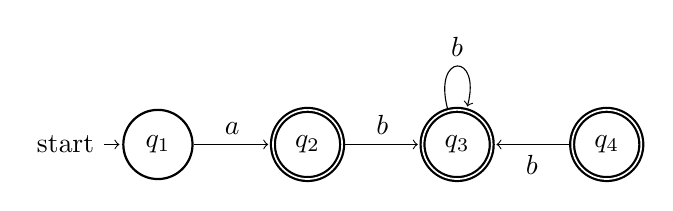
\begin{tikzpicture}[scale=0.5,node distance=1.9cm,shorten >=1pt,auto]
\node[state,initial]   (q_1)                {$q_1$};
\node[state,accepting] (q_2) [right of=q_1] {$q_2$};
\node[state,accepting] (q_3) [right of=q_2] {$q_3$};
\node[state,accepting] (q_4) [right of=q_3] {$q_4$};

\path[->]	(q_1) 	edge 			node {$a$} 		(q_2)
		(q_2)	edge 			node {$b$}		(q_3)
		(q_3)	edge [loop above]	node {$b$}		()
		(q_4)	edge			node {$b$}		(q_3);
\end{tikzpicture}
\end{center}
\end{figure}
\end{block}
Kann $A$ auf einen Automaten $A' = (Q', \Sigma, \delta', s', F')$ mit $L(A) = L(A')$ und $|Q'| < |Q|$ überführt werden?
\end{frame}
\begin{frame}
\frametitle{Minimierung von DEAs}
$q_4$ ist nicht vom Startzustand aus erreichbar
\begin{block}{Entferne \(q_4\)}
 \begin{figure}[h]
\begin{center}
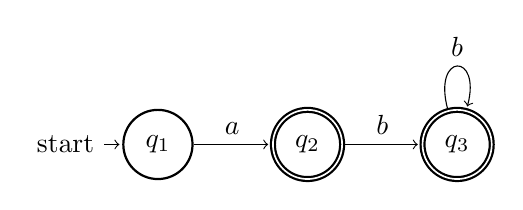
\begin{tikzpicture}[scale=0.5,node distance=1.9cm,shorten >=1pt,auto]
\node[state,initial]   (q_1)                {$q_1$};
\node[state,accepting] (q_2) [right of=q_1] {$q_2$};
\node[state,accepting] (q_3) [right of=q_2] {$q_3$};

\path[->]	(q_1) 	edge 			node {$a$} 		(q_2)
		(q_2)	edge 			node {$b$}		(q_3)
		(q_3)	edge [loop above]	node {$b$}		();
\end{tikzpicture}
\end{center}
\end{figure}
\end{block}
\pause
Schon minimal?
\end{frame}
\begin{frame}
 \frametitle{Minimierung von DEAs}
Nein!
\begin{block}{Automat \(A'' = (Q'', \Sigma, \delta'', s, F'')\)}
 \begin{figure}[H]
\begin{center}
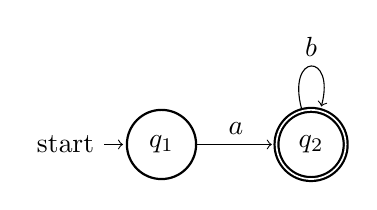
\begin{tikzpicture}[scale=0.6,node distance=1.9cm,shorten >=1pt,auto]
\node[state,initial]   (q_1)                {$q_1$};
\node[state,accepting] (q_2) [right of=q_1] {$q_2$};

\path[->]	(q_1) 	edge 			node {$a$} 		(q_2)
		(q_2)	edge [loop above]	node {$b$}		();
\end{tikzpicture}
\end{center}
\end{figure}
\end{block}
\begin{block}{}
 Akzeptierte Sprache: \(L(A) = L(A') = L(A'') = L(ab^*) \)
\end{block}
\end{frame}
\begin{frame}
 \frametitle{Methodischer Ansatz}
 \begin{block}{Definition}
  Zustände eines (deterministischen) endlichen Automaten, die vom Anfangszustand aus nicht erreichbar sind, heißen überflüssig.
 \end{block}
\begin{block}{Vorgehen}
 \begin{enumerate}
  \item Tiefensuche durchführen, um überflüssige Zustände zu finden.
  \item Diese entfernen.
  \item Aus restlichen Zuständen den Äquivalenzklassenautomaten bilden.
 \end{enumerate}
\end{block}
\end{frame}

\subsection{Äquivalenzklassenautomat}

\begin{frame}
 \frametitle{Äquivalenz}
 \begin{block}{Aus der Vorlesung}
  \begin{itemize}
   \item Zwei Zustände haben dasselbe Akzeptanzverhalten, wenn es für das Erreichen eines Endzustandes durch Abarbeiten eines Wortes $w$
   unerheblich ist, aus welchem der beiden Zustände wir starten.
  \end{itemize}
 \end{block}
 \begin{block}{Definition (Äquivalenz):}
  Zwei Zustände $p$ und $q$ eines deterministischen endlichen Automaten heißen \emph{äquivalent} ($p \equiv q$),
  wenn für alle Wörter $w\in\Sigma^*$ gilt:
  \[
   \delta(p, w)\in F \Leftrightarrow \delta(q, w)\in F
  \]
  Offensichtlich ist $\equiv$ eine Äquivalenzrelation. Mit $[p]$ bezeichnen wir die Äquivalenzklasse der zu $p$ äquivalenten Zustände.
 \end{block}
\end{frame}
\begin{frame}
 \frametitle{Beispiel}
 \begin{block}{Zurück zu $Q'$}
 \begin{figure}[h]
\begin{center}
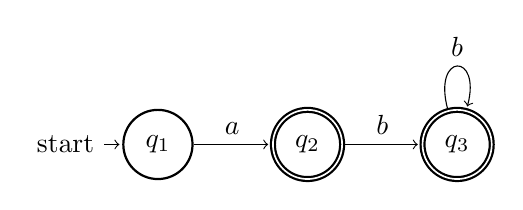
\begin{tikzpicture}[scale=0.5,node distance=1.9cm,shorten >=1pt,auto]
\node[state,initial]   (q_1)                {$q_1$};
\node[state,accepting] (q_2) [right of=q_1] {$q_2$};
\node[state,accepting] (q_3) [right of=q_2] {$q_3$};

\path[->]	(q_1) 	edge 			node {$a$} 		(q_2)
		(q_2)	edge 			node {$b$}		(q_3)
		(q_3)	edge [loop above]	node {$b$}		();
\end{tikzpicture}
\end{center}
\end{figure}
Hier sind $q_2$ und $q_3$ äquivalent. Warum?
\end{block}
\end{frame}
\begin{frame}
 \frametitle{Äquivalenzklassenautomat}
 \begin{block}{Definition aus der Vorlesung (Äquivalenzklassenautomat)}
  Zu einem DEA \(A = (Q, \Sigma, \delta, s, F)\) definieren wir den Äquivalenzklassenautomaten 
  \(A^\equiv = (Q^\equiv, \Sigma^\equiv, \delta^\equiv, s^\equiv, F^\equiv)\) durch:
  \begin{itemize}
   \item $Q^\equiv := \menge{[q]}{q\in Q}$
   \item $\Sigma^\equiv := \Sigma$
   \item $\delta^\equiv([q], a) := [\delta(q, a)]$
   \item $s^\equiv := [s]$
   \item $F^\equiv:= \menge{[f]}{f\in F}$
  \end{itemize}
 \end{block}
\end{frame}
\begin{frame}
 \frametitle{Konstruktion der Äquivalenzklassen}
 \begin{block}{}
  \begin{enumerate}
   \item Fasse alle Zustände $q_i \in Q$ in einer Klasse zusammen.
   \item $\varepsilon$ trennt Zustände aus $F$ von denen aus $Q \setminus F$.
   \item Für Worte $w\in \Sigma^*$ mit wachsender Länge und Zustandspaare $p, q$ in einer Klasse: 
    \begin{enumerate}
    \item Falls $[\delta(p, w)] \neq [\delta(q, w)]$, trenne die Zustände $q$ und $p$ ($w$ ist Zeuge).
    \item Brich ab, falls sich für eine Wortlänge keine weiteren Zeugen finden.
    \end{enumerate}
  \end{enumerate}
 \end{block}
 \pause
 \begin{block}{Toller:}
   \begin{enumerate}
    \setcounter{enumi}{2}
    \item Für Zeichen $x \in \Sigma$ und Zustandspaare $p, q$ in einer Klasse:
     \begin{enumerate}
     \item Falls $[\delta(p, x)] \neq [\delta(q, x)]$, trenne die Zustände $q$ und $p$ .
     \item Brich ab, falls in einem Durchlauf kein Zeichen mehr Zustände trennt.
     \end{enumerate}
   \end{enumerate}
  \end{block}
\end{frame}
\frame{
  \frametitle{Automaten-Minimierung: Beispiel}
  \begin{figure}[H]
  \begin{center}
  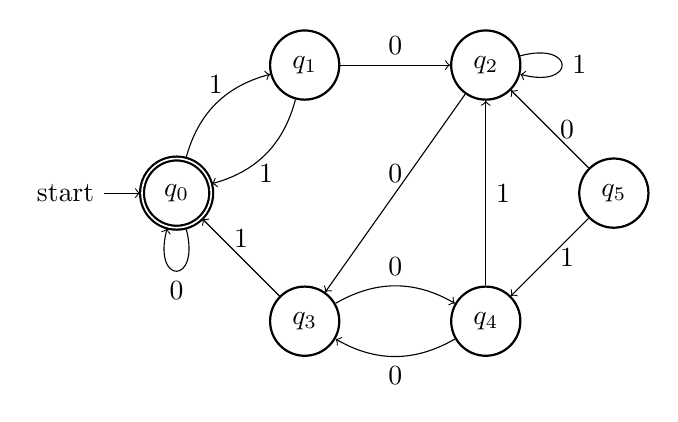
\begin{tikzpicture}[node distance=2.3cm]
  \tikzstyle{normal}=[draw]


  \node[state,accepting,initial]  (q0)                      {$q_0$};
  \node[state]         (q1)  [above right of=q0] {$q_1$};
  \node[state]         (q2)  [right of=q1]       {$q_2$};
  \node[state]         (q3)  [below right of=q0] {$q_3$};
  \node[state]         (q4)  [right of=q3]       {$q_4$};
  \node[state]         (q5)  [above right of=q4] {$q_5$};
  
  \draw[->,bend left] (q0)  to node[above] {1} (q1);
  \draw[->,loop below] (q0)  to node [below] {0} (q0);

  \draw[->,bend left] (q1)  to node[below] {1} (q0);
  \draw[->] (q1)  to node[above] {0} (q2);

  \draw[->] (q2) to node[above] {0} (q3);
  \draw[->,loop right] (q2) to node[right] {1} (q2);

  \draw[->] (q3)  to node[above] {1} (q0);
  \draw[->,bend left] (q3)  to node[above] {0} (q4);
  
  \draw[->,bend left] (q4)  to node[below] {0} (q3);
  \draw[->] (q4)  to node[right] {1} (q2);

  \draw[->] (q5)  to node[right] {0} (q2);
  \draw[->] (q5)  to node[right] {1} (q4);
  \end{tikzpicture}
  \end{center}
  \end{figure}
}
\begin{frame}
 \frametitle{Automaten-Minimierung: Aufgabe}
Konstruiere zu folgendem DEA den Äquivalenzklassenautomaten:

 \begin{figure}[H]
  \begin{center}
  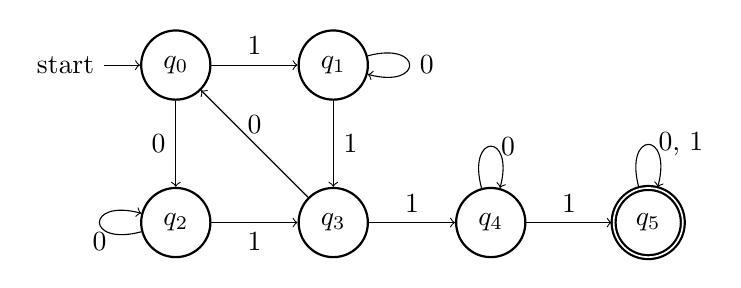
\begin{tikzpicture}[node distance=2cm]
  \tikzstyle{normal}=[draw]


  \node[state,initial]         (q0)                      {$q_0$};
  \node[state]         (q1)  [right of=q0] {$q_1$};
  \node[state]         (q2)  [below of=q0]       {$q_2$};
  \node[state]         (q3)  [right of=q2] {$q_3$};
  \node[state]         (q4)  [right of=q3]       {$q_4$};
  \node[state,accepting]         (q5)  [right of=q4] {$q_5$};

  \draw[->] (q0)  to node[above] {1} (q1);
  \draw[->] (q0)  to node [left] {0} (q2);

  \draw[->,loop right] (q1)  to node[right] {0} (q0);
  \draw[->] (q1)  to node[right] {1} (q3);

  \draw[->] (q2) to node[below] {1} (q3);
  \draw[->,loop left] (q2) to node[below] {0} (q2);

  \draw[->] (q3)  to node[above] {1} (q4);
  \draw[->] (q3)  to node[above] {0} (q0);
  
  \draw[->,loop above] (q4)  to node[right] {0} (q4);
  \draw[->] (q4)  to node[above] {1} (q5);

  \draw[->,loop above] (q5)  to node[right] {0, 1} (q2);
  \end{tikzpicture}
  \end{center}
  \end{figure}
\end{frame}

\section{Wiederholung}
\subsection{DEAs}

\begin{frame}
\frametitle{Aufgabe zu DEAs}
Gegeben sei ein DEA (als Graph mit beschrifteten Knoten und Kanten) ohne überflüssige Zustände.
Schreibe einen Algorithmus, der entscheidet, ob die zugehörige Sprache unendlich viele Wörter hat. Hinweis: Siehe Beweis zur Korrektheit des Pumping-Lemmas.
\end{frame}



\subsection{Reguläre Sprachen}

\begin{frame}
\frametitle{Aufgabe: Regularität}

\begin{block}{Definition}
Ein Wort $w$ ist \emph{Präfix} eines Wortes
$w'$, falls ein Wort $v$ mit $wv = w'$ existiert. Gilt zusätzlich $w\neq w'$, so ist $w$ ein \emph{echtes Präfix} von $w'$.
\end{block}

\pause

\begin{block}{Aufgabe}
Sei $L$ eine reguläre Sprache. Zeige, dass dann auch die folgenden beiden Sprachen regulär sind:
\begin{enumerate}
\item NOPREFIX$(L):=\menge{w\in L}{\mbox{kein $w'\in L$ ist echtes Präfix
    von $w$}}.$
\item NOEXTEND$(L):=$ \\ \raggedleft{ $ \menge{w\in L}{\mbox{$w$ ist kein echtes Präfix eines Wortes $w'\in L$}}.$ }
\end{enumerate}
\end{block}

\pause

\begin{block}{Zur Veranschaulichung}
$ L = \left\lbrace \text{ Katze, Kater, Katzenpfote, Katzenfutter } \right\rbrace $

Was sind hier NOPREFIX$(L)$ und NOEXTEND$(L)$?
\end{block}

\end{frame}
\begin{frame}
 \frametitle{Aufgabe: Regularität}
 Zeige, dass die folgende Sprache nicht regulär ist:
 $$L = \menge{0^m 1^n}{m \neq n}$$
\end{frame}

\section{Schluss}
\subsection{Schluss}

\begin{frame}
 \frametitle{Bis zum nächsten Mal!}
 \begin{center} 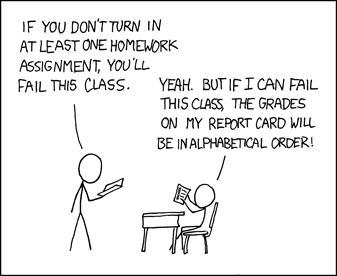
\includegraphics[scale=0.5]{images/xkcd_336.png} \end{center}
 \begin{quote}\scriptsize{You should start giving out 'E's so I can spell FACADE or DEFACED.}\end{quote}
\end{frame}

\frame{
  \frametitle{Lizenzen}
  \center
  
\includegraphics[width=2em]{images/by}
  
\includegraphics[width=2em]{images/cc}
  
\includegraphics[width=2em]{images/sa}
  \\
  {\tiny

Dieses Werk ist unter einem ``Creative Commons Namensnennung-Weitergabe unter gleichen Bedingungen 3.0 Deutschland``-Lizenzvertrag lizenziert. Um eine Kopie der Lizenz zu erhalten, gehen Sie bitte zu \href{http://creativecommons.org/licenses/by-sa/3.0/de/}{http://creativecommons.org/licenses/by-sa/3.0/de/} oder schreiben Sie an Creative Commons, 171 Second Street, Suite 300, San Francisco, California 94105, USA.\\
  \vspace{1cm}
  Davon ausgenommen sind das Titelbild, welches aus der März-April 2002 Ausgabe von American Scientist erschienen ist und ohne Erlaubnis verwendet wird, sowie das KIT Beamer Theme. Hierfür gelten die Bestimmungen der jeweiligen Urheber.
  \vspace{1cm}
  \\ 
  }
  %Habe hier die Reihenfolge etwas umgestellt, weil die Formatierung bei mir komisch aussah. 
  %Wenn es bei dir anders ist, kannst du es auch wieder zurückändern, dann haben wir unterschiedliche Kompilieroptionen
}

\end{document}
